\documentclass[english,11pt,table,handout]{beamer}

% Copyright 2007 by Till Tantau
%
% This file may be distributed and/or modified
%
% 1. under the LaTeX Project Public License and/or
% 2. under the GNU Public License.
%
% See the file doc/licenses/LICENSE for more details.


% Common packages
\usepackage[utf8x]{inputenc}
\usepackage[vietnam,english]{babel}
\usepackage[utf8]{vietnam}
%\usepackage{times}
\usefonttheme[onlymath]{serif}
\usecolortheme{default}
\usepackage{booktabs}
\usepackage{mathpartir}
\usepackage{listings}
\usepackage{listingsutf8}

\usepackage{pbox}
\mprset{flushleft}
\mode<article>
{
  \usepackage{times}
  \usepackage{mathptmx}
  \usepackage[left=1.5cm,right=6cm,top=1.5cm,bottom=3cm]{geometry}
}

\usepackage{hyperref}
\usepackage{tikz}
\usetikzlibrary{arrows,backgrounds}
%\tikzstyle{mnode}=[circle, draw, fill=black, inner sep=0pt, minimum width=4pt]
\usepackage{colortbl}
%\usepackage{yfonts}
\usepackage{translator} % comment this, if not available


% Common settings for all lectures in this course

\def\lecturename{Image Processing and Computer Vision}

\title{\insertlecture}

\author{\textbf{LE Thanh Sach}}

\institute
{
  \textit{Faculty of Computer Science and Engineering}\\
  \textit{Ho Chi Minh University of Technology, VNU-HCM}
}

\subject{Lecturer \lecturename}

% Beamer version theme settings

\useoutertheme[height=0pt,width=2cm,right]{sidebar}
\usecolortheme{rose,sidebartab}
\useinnertheme{circles}
\usefonttheme[only large]{structurebold}

\setbeamercolor{sidebar right}{bg=black!15}
\setbeamercolor{structure}{fg=blue}
\setbeamercolor{author}{parent=structure}

\setbeamerfont{title}{series=\normalfont,size=\LARGE}
\setbeamerfont{title in sidebar}{series=\bfseries}
\setbeamerfont{author in sidebar}{series=\bfseries}
\setbeamerfont*{item}{series=}
\setbeamerfont{frametitle}{size=}
\setbeamerfont{block title}{size=\small}
\setbeamerfont{subtitle}{size=\normalsize,series=\normalfont}

\setbeamertemplate{navigation symbols}{}
\setbeamertemplate{bibliography item}[book]
\setbeamertemplate{sidebar right}
{
  {\usebeamerfont{title in sidebar}%
    \vskip1.5em%
    \hskip3pt%
    \usebeamercolor[fg]{title in sidebar}%
    \insertshorttitle[width=2cm,center,respectlinebreaks]\par%
    \vskip1.25em%
  }%
  {%
    \hskip3pt%
    \usebeamercolor[fg]{author in sidebar}%
    \usebeamerfont{author in sidebar}%
    \insertshortauthor[width=2cm,center,respectlinebreaks]\par%
    \vskip1.25em%
  }%
  \hbox to2cm{\hss\insertlogo\hss}
  \vskip1.25em%
  \insertverticalnavigation{2cm}%
  \vfill
  \hbox to 2cm{\hfill\usebeamerfont{subsection in
      sidebar}\strut\usebeamercolor[fg]{subsection in
      sidebar}\insertshortlecture.\insertframenumber\hskip5pt}%
  \vskip3pt%
}%

\setbeamertemplate{title page}
{
  \vbox{}
  \vskip1em
  {\huge Chapter \insertshortlecture\par}
  {\usebeamercolor[fg]{title}\usebeamerfont{title}\inserttitle\par}%
  \ifx\insertsubtitle\@empty%
  \else%
    \vskip0.25em%
    {\usebeamerfont{subtitle}\usebeamercolor[fg]{subtitle}\insertsubtitle\par}%
  \fi%     
  \vskip1em\par
  \emph{\lecturename}\ 
  %on \insertdate\par
  \vskip3em\par

  \leftskip=0pt plus1fill\insertauthor\par
  \insertinstitute\vskip1em
}

\logo{
\includegraphics[width=1.5cm]{hcmut.png}}



% Article version layout settings

\mode<article>

\makeatletter
\def\@listI{\leftmargin\leftmargini
  \parsep 0pt
  \topsep 5\p@   \@plus3\p@ \@minus5\p@
  \itemsep0pt}
\let\@listi=\@listI


\setbeamertemplate{frametitle}{\paragraph*{\insertframetitle\
    \ \small\insertframesubtitle}\ \par
}
\setbeamertemplate{frame end}{%
  \marginpar{\scriptsize\hbox to 1cm{\sffamily%
      \hfill\strut\insertshortlecture.\insertframenumber}\hrule height .2pt}}
\setlength{\marginparwidth}{1cm}
\setlength{\marginparsep}{4.5cm}

\def\@maketitle{\makechapter}

\def\makechapter{
  \newpage
  \null
  \vskip 2em%
  {%
    \parindent=0pt
    \raggedright
    \sffamily
    \vskip8pt
    {\fontsize{36pt}{36pt}\selectfont Chapter \insertshortlecture \par\vskip2pt}
    {\fontsize{24pt}{28pt}\selectfont \color{blue!50!black} \insertlecture\par\vskip4pt}
    {\Large\selectfont \color{blue!50!black} \insertsubtitle\par}
    \vskip10pt

    \normalsize\selectfont Print version of
    Lecturer \emph{\lecturename} of \@date\par\vskip1.5em
    %\hfill Le Thanh Sach and Luong The Nhan, Faculty of CSE, HCMC University of Technology
  }
  \par
  \vskip 1.5em%
}

\let\origstartsection=\@startsection
\def\@startsection#1#2#3#4#5#6{%
  \origstartsection{#1}{#2}{#3}{#4}{#5}{#6\normalfont\sffamily\color{blue!50!black}\selectfont}}

\makeatother

\mode
<all>




% Typesetting Listings

\usepackage{listings}
\lstset{language=Java}

\alt<presentation>
{\lstset{%
  basicstyle=\footnotesize\ttfamily,
  commentstyle=\slshape\color{green!50!black},
  keywordstyle=\bfseries\color{blue!50!black},
  identifierstyle=\color{blue},
  stringstyle=\color{orange},
  escapechar=\#,
  emphstyle=\color{red}}
}
{
  \lstset{%
    basicstyle=\ttfamily,
    keywordstyle=\bfseries,
    commentstyle=\itshape,
    escapechar=\#,
    emphstyle=\bfseries\color{red}
  }
}



% Common theorem-like environments

\theoremstyle{example}
\newtheorem{exercise}[theorem]{\translate{Exercise}}


% New useful definitions:

\newbox\mytempbox
\newdimen\mytempdimen

\newcommand\includegraphicscopyright[3][]{%
  \leavevmode\vbox{\vskip3pt\raggedright\setbox\mytempbox=\hbox{\includegraphics[#1]{#2}}%
    \mytempdimen=\wd\mytempbox\box\mytempbox\par\vskip1pt%
    \fontsize{3}{3.5}\selectfont{\color{black!25}{\vbox{\hsize=\mytempdimen#3}}}\vskip3pt%
}}

\newenvironment{colortabular}[1]{\medskip\rowcolors[]{1}{blue!20}{blue!10}\tabular{#1}\rowcolor{blue!40}}{\endtabular\medskip}

\def\equad{\leavevmode\hbox{}\quad}

\newenvironment{greencolortabular}[1]
{\medskip\rowcolors[]{1}{green!50!black!20}{green!50!black!10}%
  \tabular{#1}\rowcolor{green!50!black!40}}%
{\endtabular\medskip}
\usepackage{pgf}

\newcommand{\Rule}[2]{\genfrac{}{}{0.7pt}{}{{\setlength{\fboxrule}{0pt}\setlength{\fboxsep}{3mm}\fbox{$#1$}}}{{\setlength{\fboxrule}{0pt}\setlength{\fboxsep}{3mm}\fbox{$#2$}}}}

\newcommand{\Rulee}[3]{\genfrac{}{}{0.7pt}{}{{\setlength{\fboxrule}{0pt}\setlength{\fboxsep}{3mm}\fbox{$#1$}}}{{\setlength{\fboxrule}{0pt}\setlength{\fboxsep}{3mm}\fbox{$#2$}}}[#3]}

\usepackage{url}

\usepackage{qtree}

\usepackage{datetime}

\usepackage{amsfonts}
\usepackage{mathtools}
\usepackage{fancybox}
\usepackage[linesnumbered]{algorithm2e}
\usepackage{ragged2e}
\usepackage{nicefrac}
\usepackage{accents}


\lecture[1]{Introduction}{lecture-text}

% \subtitle{Sequence Control}

\date{09 September 2015}
\newcounter{saveenumi}

\usepackage{wrapfig}
\usetikzlibrary{automata,arrows,positioning, chains, shapes.callouts, calc}

\tikzstyle{mnode}=[circle, draw, fill=black, inner sep=0pt, minimum width=4pt]
\tikzstyle{thinking} = [draw=blue, very thick]
\edef\sizetape{1cm}
\tikzstyle{tmtape}=[draw,minimum size=\sizetape]
\tikzstyle{tmhead}=[arrow box,draw,minimum size=.5cm,arrow box
arrows={east:.25cm, west:0.25cm}]
\tikzset{
  level/.style   = { ultra thick, blue },
  connect/.style = { dashed, red },
  notice/.style  = { draw, rectangle callout, callout relative pointer={#1} },
  label/.style   = { text width=4cm }
}

\begin{document}

\begin{frame}
\selectlanguage{english}
  \maketitle
\end{frame}

\begin{frame}\frametitle<presentation>{Overview}
  \tableofcontents
\end{frame}

%%%%%%%%%%%%%%%%%%%%%%%%%%%%%%%%%%%%%%%%%%%%%%%%%%%%%%%%%%%%%%%%%%%%%
%%%%%%%%%%%%%%%%%%%%%%%%%%%%%%%%%%%%%%%%%%%%%%%%%%%%%%%%%%%%%%%%%%%%%

\section{Linear Filters}
\frame
{
	\Huge
	\begin{center}
	\textcolor{blue}{\textbf{Linear Filters}}
	\end{center}
}
\section{Non-Linear Filters}
\frame
{
	\Huge
	\begin{center}
		\textcolor{blue}{\textbf{Non-Linear Filters}}
	\end{center}
}
\section{Noise's Model}
\frame
{
	\Huge
	\begin{center}
		\textcolor{blue}{\textbf{Noise's Model}}
	\end{center}
}
\subsection{Sources of Noise}
\frame
{
	\frametitle{Sources of noise}
	\begin{block}{Sources of noise}
		\begin{enumerate}
			\item Environmental conditions during image acquisition.
				\begin{itemize}
					\item Light level
					\item Sensor temperature
					
				\end{itemize}
			\item Transmission
				\begin{itemize}
					\item Signal interference
					\item Quality of transmission channels
					
				\end{itemize}
		\end{enumerate}
	\end{block}
}

\subsection{Types of Noise}
\frame
{
	\frametitle{Gaussian Noise}
	\begin{block}{Gaussian probability density function}
		For each pixel in $I(u,v)$, the noise value $z$ is drawn from a Gaussian probability density function.
		
		\begin{align}
		\nonumber
			p(z) &= \frac{1}{\sqrt{(2\pi)}\sigma}e^{-\frac{(z-\mu)^2}{2\sigma^2}}
		\end{align}
		\begin{enumerate}
			\item $\mu$ : the mean of noise values, i.e., $z$
			\item $\sigma$ : the standard deviation.
			\item $\sigma^2$ : the variance of $z$
		\end{enumerate}
		
	\end{block}

}

\frame
{
	\frametitle{Gaussian Noise}
	\begin{figure}[!h]
		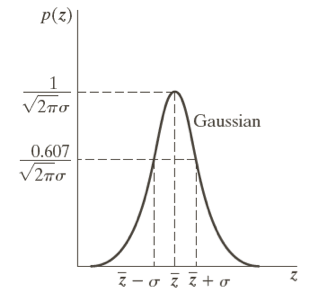
\includegraphics[scale=1.0]{gaussian_1d.png}
	\end{figure}
	
	\begin{alertblock}{Properties}
		\begin{enumerate}
			\item $[\mu - \sigma, \mu + \sigma]$ : contains approximately $70\%$ of noise values
			\item $[\mu - 2\sigma, \mu + 2\sigma]$ : contains approximately $95\%$ of noise values
		\end{enumerate}
	\end{alertblock}
}
\frame
{
	\frametitle{Rayleigh Noise}
	\begin{block}{Rayleigh probability density function}
		For each pixel in $I(u,v)$, the noise value $z$ is drawn from a Rayleigh probability density function.
		
		$$
			p(z) =
				\begin{cases}
					\frac{2}{b}(z-a)e^{-(z-a)^{2}/b} & \text{for } z \ge a\\
					0 & \text{for } z < a\\
				\end{cases}
		$$
	
		\begin{enumerate}
			\item \alert{\textbf{mean of noises}}: 
				\begin{align}
					\nonumber
					\mu = a + \sqrt{\pi b/4}
				\end{align}
			\item \alert{\textbf{variance of noises}}:
				\begin{align}
				\nonumber
					\sigma^2 = \frac{b(4-\pi)}{4}
				\end{align}
		\end{enumerate}
		
	\end{block}
	
}
\frame
{
	\frametitle{Rayleigh Noise}
	\begin{figure}[!h]
		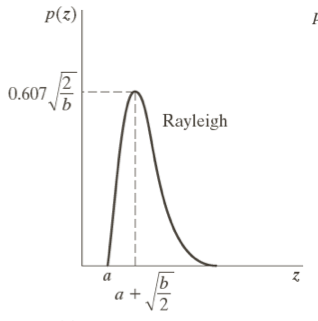
\includegraphics[scale=1.0]{rayleigh_1d.png}
	\end{figure}
	
	\begin{alertblock}{Properties}
		\begin{enumerate}
			\item The minimum noise value is $a$
			\item The density is skewed to the right
			\item $b > 0$
		\end{enumerate}
	\end{alertblock}
}

\frame
{
	\frametitle{Erlang (Gamma) Noise}
	\begin{block}{Erlang probability density function}
		For each pixel in $I(u,v)$, the noise value $z$ is drawn from a Erlang probability density function.
		
		$$
		p(z) =
		\begin{cases}
			\frac{a^{b}z^{b-1}}{(b-1)!} e^{-az}& \text{for } z \ge 0\\
			0 & \text{for } z < 0\\
		\end{cases}
		$$
		
		\begin{enumerate}
			\item \alert{\textbf{mean of noises}}: 
			\begin{align}
			\nonumber
			\mu = \frac{b}{a}
			\end{align}
			\item \alert{\textbf{variance of noises}}:
			\begin{align}
			\nonumber
			\sigma^2 = \frac{b}{a^2}
			\end{align}
		\end{enumerate}
		
	\end{block}
	
}
\frame
{
	\frametitle{Erlang Noise}
	\begin{figure}[!h]
		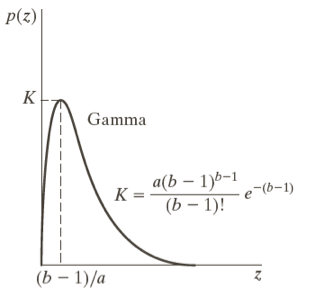
\includegraphics[scale=1.0]{erlang_1d.png}
	\end{figure}
	
	\begin{alertblock}{Properties}
		\begin{enumerate}
			\item The minimum noise value is $0$
			\item $a > 0$
			\item $b$ is a positive integer
		\end{enumerate}
	\end{alertblock}
}

\frame
{
	\frametitle{Exponential Noise}
	\begin{block}{Exponential probability density function}
		For each pixel in $I(u,v)$, the noise value $z$ is drawn from a exponential probability density function.
		
		$$
		p(z) =
		\begin{cases}
		ae^{-az}& \text{for } z \ge 0\\
		0 & \text{for } z < 0\\
		\end{cases}
		$$
		
		\begin{enumerate}
			\item \alert{\textbf{mean of noises}}: 
			\begin{align}
			\nonumber
			\mu = \frac{1}{a}
			\end{align}
			\item \alert{\textbf{variance of noises}}:
			\begin{align}
			\nonumber
			\sigma^2 = \frac{1}{a^2}
			\end{align}
		\end{enumerate}
		
	\end{block}
	
}
\frame
{
	\frametitle{Exponential Noise}
	\begin{figure}[!h]
		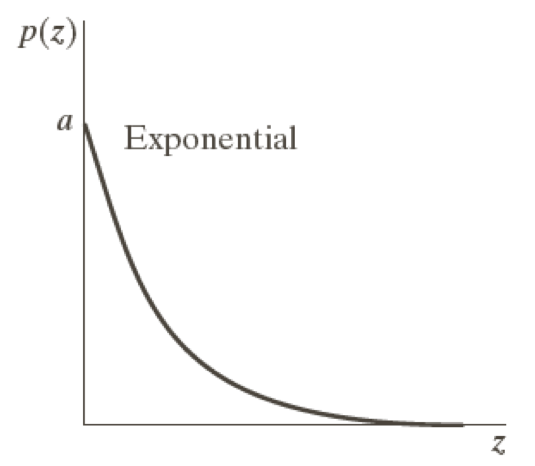
\includegraphics[scale=0.6]{exponential.png}
	\end{figure}
	
	\begin{alertblock}{Properties}
		\begin{enumerate}
			\item The minimum noise value is $0$
			\item $a > 0$
			\item Exponential noise is a special case of Erlang noise, with $b=1$		\end{enumerate}
	\end{alertblock}
}

\frame
{
	\frametitle{Uniform Noise}
	\begin{block}{Probability density function of uniform noise}
		For each pixel in $I(u,v)$, the noise value $z$ is drawn from a uniform probability density function.
		
		$$
		p(z) =
		\begin{cases}
		\frac{1}{b-a}& \text{if } a \le z \le b \\
		0 & \text{otherwise} \\
		\end{cases}
		$$
		
		\begin{enumerate}
			\item \alert{\textbf{mean of noises}}: 
			\begin{align}
			\nonumber
			\mu = \frac{a+b}{2}
			\end{align}
			\item \alert{\textbf{variance of noises}}:
			\begin{align}
			\nonumber
			\sigma^2 = \frac{(b-a)^2}{12}
			\end{align}
		\end{enumerate}
		
	\end{block}
	
}
\frame
{
	\frametitle{Uniform Noise}
	\begin{figure}[!h]
		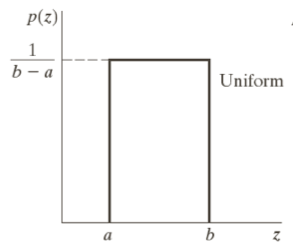
\includegraphics[scale=1.0]{uniform.png}
	\end{figure}
	
	\begin{alertblock}{Properties}
		\begin{enumerate}
			\item Noise values range from $a$ to $b$
			\item $a \le b$
			\item Probability of noise values are equal ($=\frac{1}{b-a}$).
			\end{enumerate}
	\end{alertblock}
}
\frame
{
	\frametitle{Impulse (pepper-and-salt) Noise}
	\begin{block}{Probability density function of uniform noise}
		For each pixel in $I(u,v)$, the noise value $z$ is drawn from a bipolar impulse probability density function.
		
		$$
		p(z) =
		\begin{cases}
			P_{a}& \text{for } z = a \\
			P_{b}& \text{for } z = b \\
			0 & otherwise
		\end{cases}
		$$
		
		\begin{enumerate}
			\item \alert{\textbf{Bipolar impulse}}: both of $P_a$ and $P_b$ are not zero.
			\item \alert{\textbf{Unipolar impulse}}: either $P_a$ or $P_b$ is zero.
			\item \alert{\textbf{Light vs dark dot}}: $b > a$, gray-level $b$ will appear as a light dot, gray-level $a$ will appear as a dark dot.
			
		\end{enumerate}
		
	\end{block}
	
}
\frame
{
	\frametitle{Impulse Noise}
	\begin{figure}[!h]
		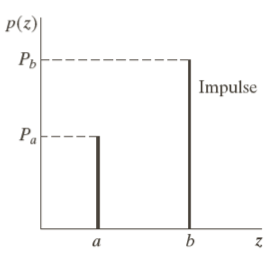
\includegraphics[scale=0.8]{impulse.png}
	\end{figure}
	
	\begin{alertblock}{Properties}
		\begin{enumerate}
			\item Impulse corruption is large; so, impulse noise should be digitalized as extreme (pure black or white)
			\item For signed numbers: negative impulse $\rightarrow$ black; positive impulse $\rightarrow$ white
			\item For unsigned 8-bit numbers: $a = 0$ (black), $b=255$ (white)
			
		\end{enumerate}
	\end{alertblock}
}

\frame
{
	\frametitle{Images with noise}
	\selectlanguage{english}
	\begin{figure}[!h]
		
\includegraphics[scale=0.8]{pattern_no_noise.jpg}
		\caption{Pattern without noise}
	\end{figure}
}
\frame
{
	\frametitle{Images with noise}
	\begin{figure}[!h]
		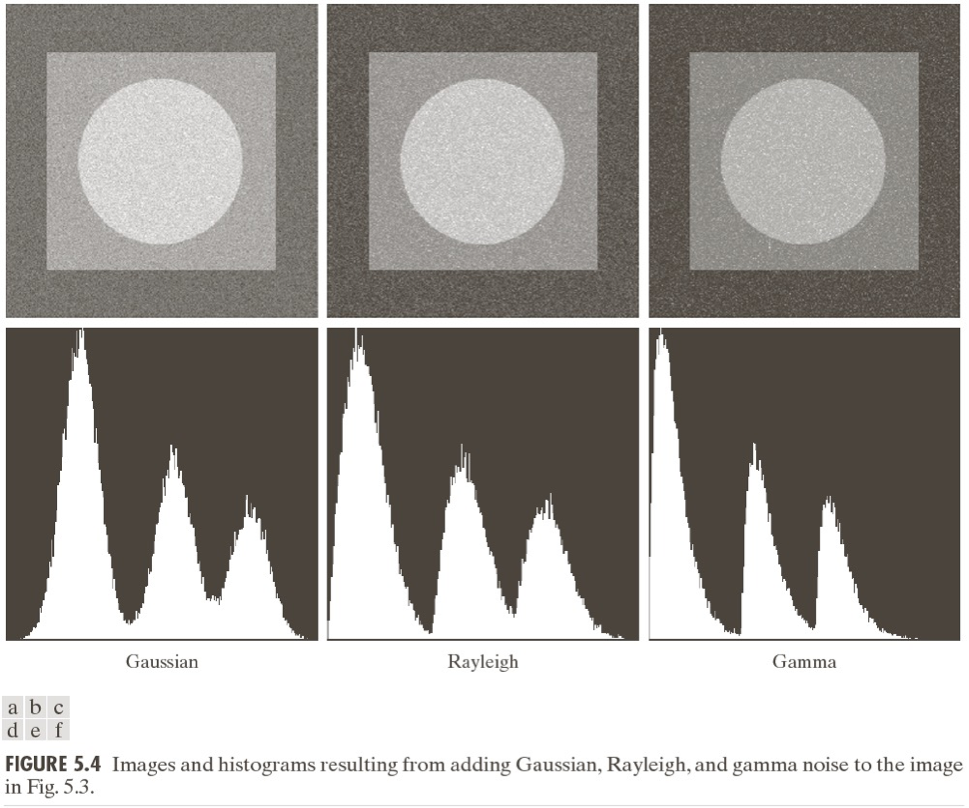
\includegraphics[scale=0.6]{im_with_noise_1.png}
	\end{figure}
}
\frame
{
	\frametitle{Images with noise}
	\begin{figure}[!h]
		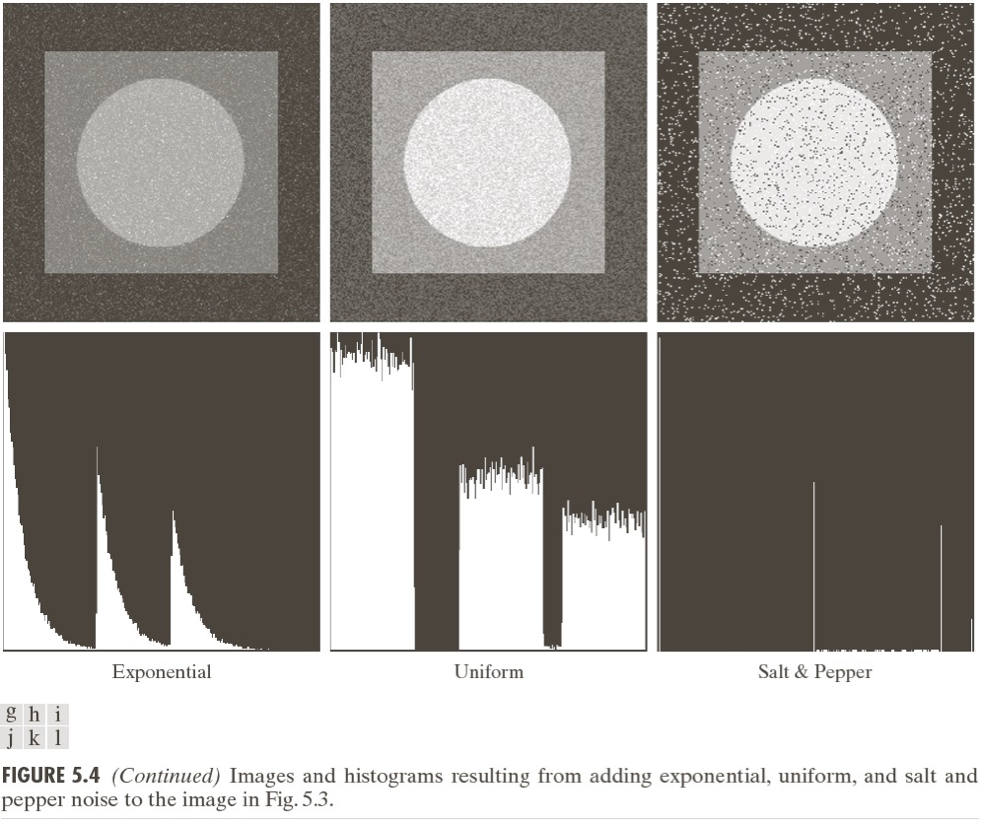
\includegraphics[scale=0.6]{im_with_noise_2.png}
	\end{figure}
}

\frame
{
	\frametitle{Periodic Noise}
	\selectlanguage{english}
	
	\begin{alertblock}{Periodic Noise}
		\begin{enumerate}
			\item \textbf{Cause}: during image acquisition
			\item \textbf{Type}: This is spatially dependent noise
		\end{enumerate}
	\end{alertblock}
	\begin{example}
		\begin{figure}[!h]
			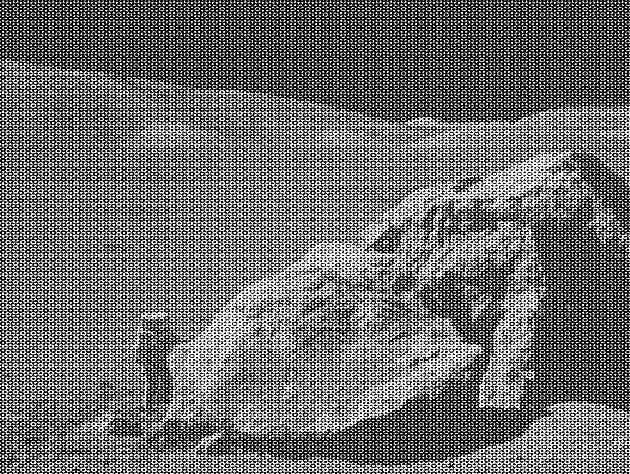
\includegraphics[scale=0.25]{periodic_noise_image.jpg}
			\caption{Example of periodic noise}
			\label{fig:periodic}
		\end{figure}
	\end{example}
}
\frame
{
	\frametitle{Periodic Noise}
	\selectlanguage{english}

	\begin{example}
		\begin{figure}[!h]
			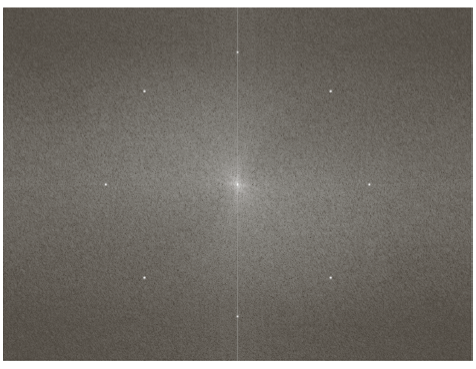
\includegraphics[scale=0.8]{periodic_freq.png}
			\caption{Frequency spectrum of previous image}
			\label{fig:periodic}
		\end{figure}
	\end{example}
}
\frame
{
	\frametitle{Periodic Noise}
	\selectlanguage{english}
	
	\begin{alertblock}{Properties}
		\begin{enumerate}
			\item Image shows periodic noise (sinusoidal) spatially.
			\item So, frequency spectrum has some bight dot at some frequencies.
			\item Therefore, this noise can be removed effectively in frequency domain.
		\end{enumerate}
	\end{alertblock}
}


\section{Noise generation}
\frame
{
	\frametitle{Noise generation}
	\selectlanguage{english}
	
	\begin{alertblock}{Why do we need to generate noise?}
		\begin{itemize}
			\item Noise is unwanted
			\item However, we need to generate them and to model them for research purpose.
		\end{itemize} 
		
	\end{alertblock}

	\begin{block}{Problem}
		Assume that we have following
		\begin{enumerate}
			\item $p_x(x)$: a probability density function of a random variable $x$
			\item $p_z(z)$: a probability density function of a random variable $z$
		\end{enumerate} 
		Can we generate variable $z$ if we have $x$, $p_x(x)$, and $p_z(z)$?
	\end{block}
}
\frame
{
	\frametitle{Noise generation}
	\selectlanguage{english}
	
	Let $c_x(x)$ and $c_z(z)$ be distribution function of variables $x$ and $z$. \newline
	$c_x(x)$ and $c_z(z)$ are cumulative density functions of $x$ and $z$. These functions can be computed as follows:

	\begin{align}
		\nonumber
		c_x(x) &= \sum_{i=-\infty}^{x}{p_x(i)}\\
		\nonumber
		c_z(z) &= \sum_{i=-\infty}^{z}{p_z(i)}
	\end{align}

}
\frame
{
	\frametitle{Noise generation}
	\selectlanguage{english}
	
	Let $z = f(x)$ be a function that map one-to-one between $x$ and $z$. We have to discover this function.
	\begin{block}{Discovering $z = f(x)$ }
		\begin{itemize}
			\item Assume that we have $z_1 = f(x_1)$ 
			\item Then, $c_z(z_1) = c_x(x_1)$. This is because of one-one mapping
			\begin{itemize}
				\item A value $x < x_1$ will be mapped into $z < z_1$
			\end{itemize}
			\item Define $w \equiv c_x(x_1)$, i.e., $w \equiv c_z(z_1) \equiv c_x(x_1)$
		\end{itemize}
		
		Therefore,
		\begin{itemize}
			\item $z_1 = c_z^{-1}(w) \equiv   c_z^{-1}(c_x(x_1))$
		\end{itemize}
	\end{block}
	\begin{alertblock}{Mapping function $f(x)$}
		\centering
		$z = f(x) =  c_z^{-1}(c_x(x))$
		
	\end{alertblock}
	

}
\frame
{
	\frametitle{Noise generation}
	\selectlanguage{english}
	
	\begin{alertblock}{Mapping function $f(x)$: Meaning}
		\centering
		$z = f(x) =  c_z^{-1}(c_x(x))$
		\begin{itemize}
			\item We can generate noise value $z$ distributed with PDF $p_z(z)$, if we has input value $x$ distributed with PDF $p_x(x)$
		\end{itemize}
		\flushleft
		\alert{\textbf{Why?}}
		\newline
		\alert{\textbf{Because,}}
		\begin{itemize}
			\item If we know PDF $p_x(x)$, we can compute $c_x(x)$.
			\item If we know PDF $p_z(z)$, we can compute $c_z(z)$.
			\item From $c_z(z)$, we can obtain $c_z^{-1}(z)$ in term of closed-form or in term of a look-up table.
		\end{itemize}
	\end{alertblock}
	
	\begin{alertblock}{}
		This is idea is also applied to Histogram equalization and matching
	\end{alertblock}	
}

\frame
{
	\frametitle{Noise generation}
	\selectlanguage{english}
	
	\begin{block}{Some random number generators}
		Almost programming languages provide function \alert{\textbf{rand()}} and \alert{\textbf{randn()}} to generate number distributed with uniform or Gaussian probability density function respectively.
		
		Therefore,
		We can use these function to generate $x$ and then from $x$ to generate noise $z$ with other kinds distributions.
	\end{block}
	

	
}

\frame
{
	\frametitle{Noise generation}
	\selectlanguage{english}
	
	\begin{block}{How do we compute generate $y$ in practice?}
		\begin{enumerate}
			\item Generate random variable $x$ by uniform distribution. Existing function $rand(.)$ in many programming language can do this task
			\item Compute $w = c_x(x)$. Please note that $c_x(x)$ is uniform distribution function.
			\item If we have closed-form of $z = c_z^{-1}(w)$ then can use this function to determine $z$.
			\item If we do not have closed-form of $c_z^{-1}(z)$
			\begin{itemize}
				\item Create a lookup table at the beginning for mapping $z \rightarrow c_z^{-1}(p)$, for discrete values $p$. We can do this because we know $c_z(z)$ in advance. This task is equal to rasterize $p = c_z(z)$ and store pairs into lookup table
				\item Determine $z$ according to the lookup table.
			\end{itemize} 
			
		\end{enumerate}
		
	\end{block}
}

\frame
{
	\frametitle{Noise generation: some popular PDF and CDF functions}
	\selectlanguage{english}
	
	\begin{figure}[!h]
		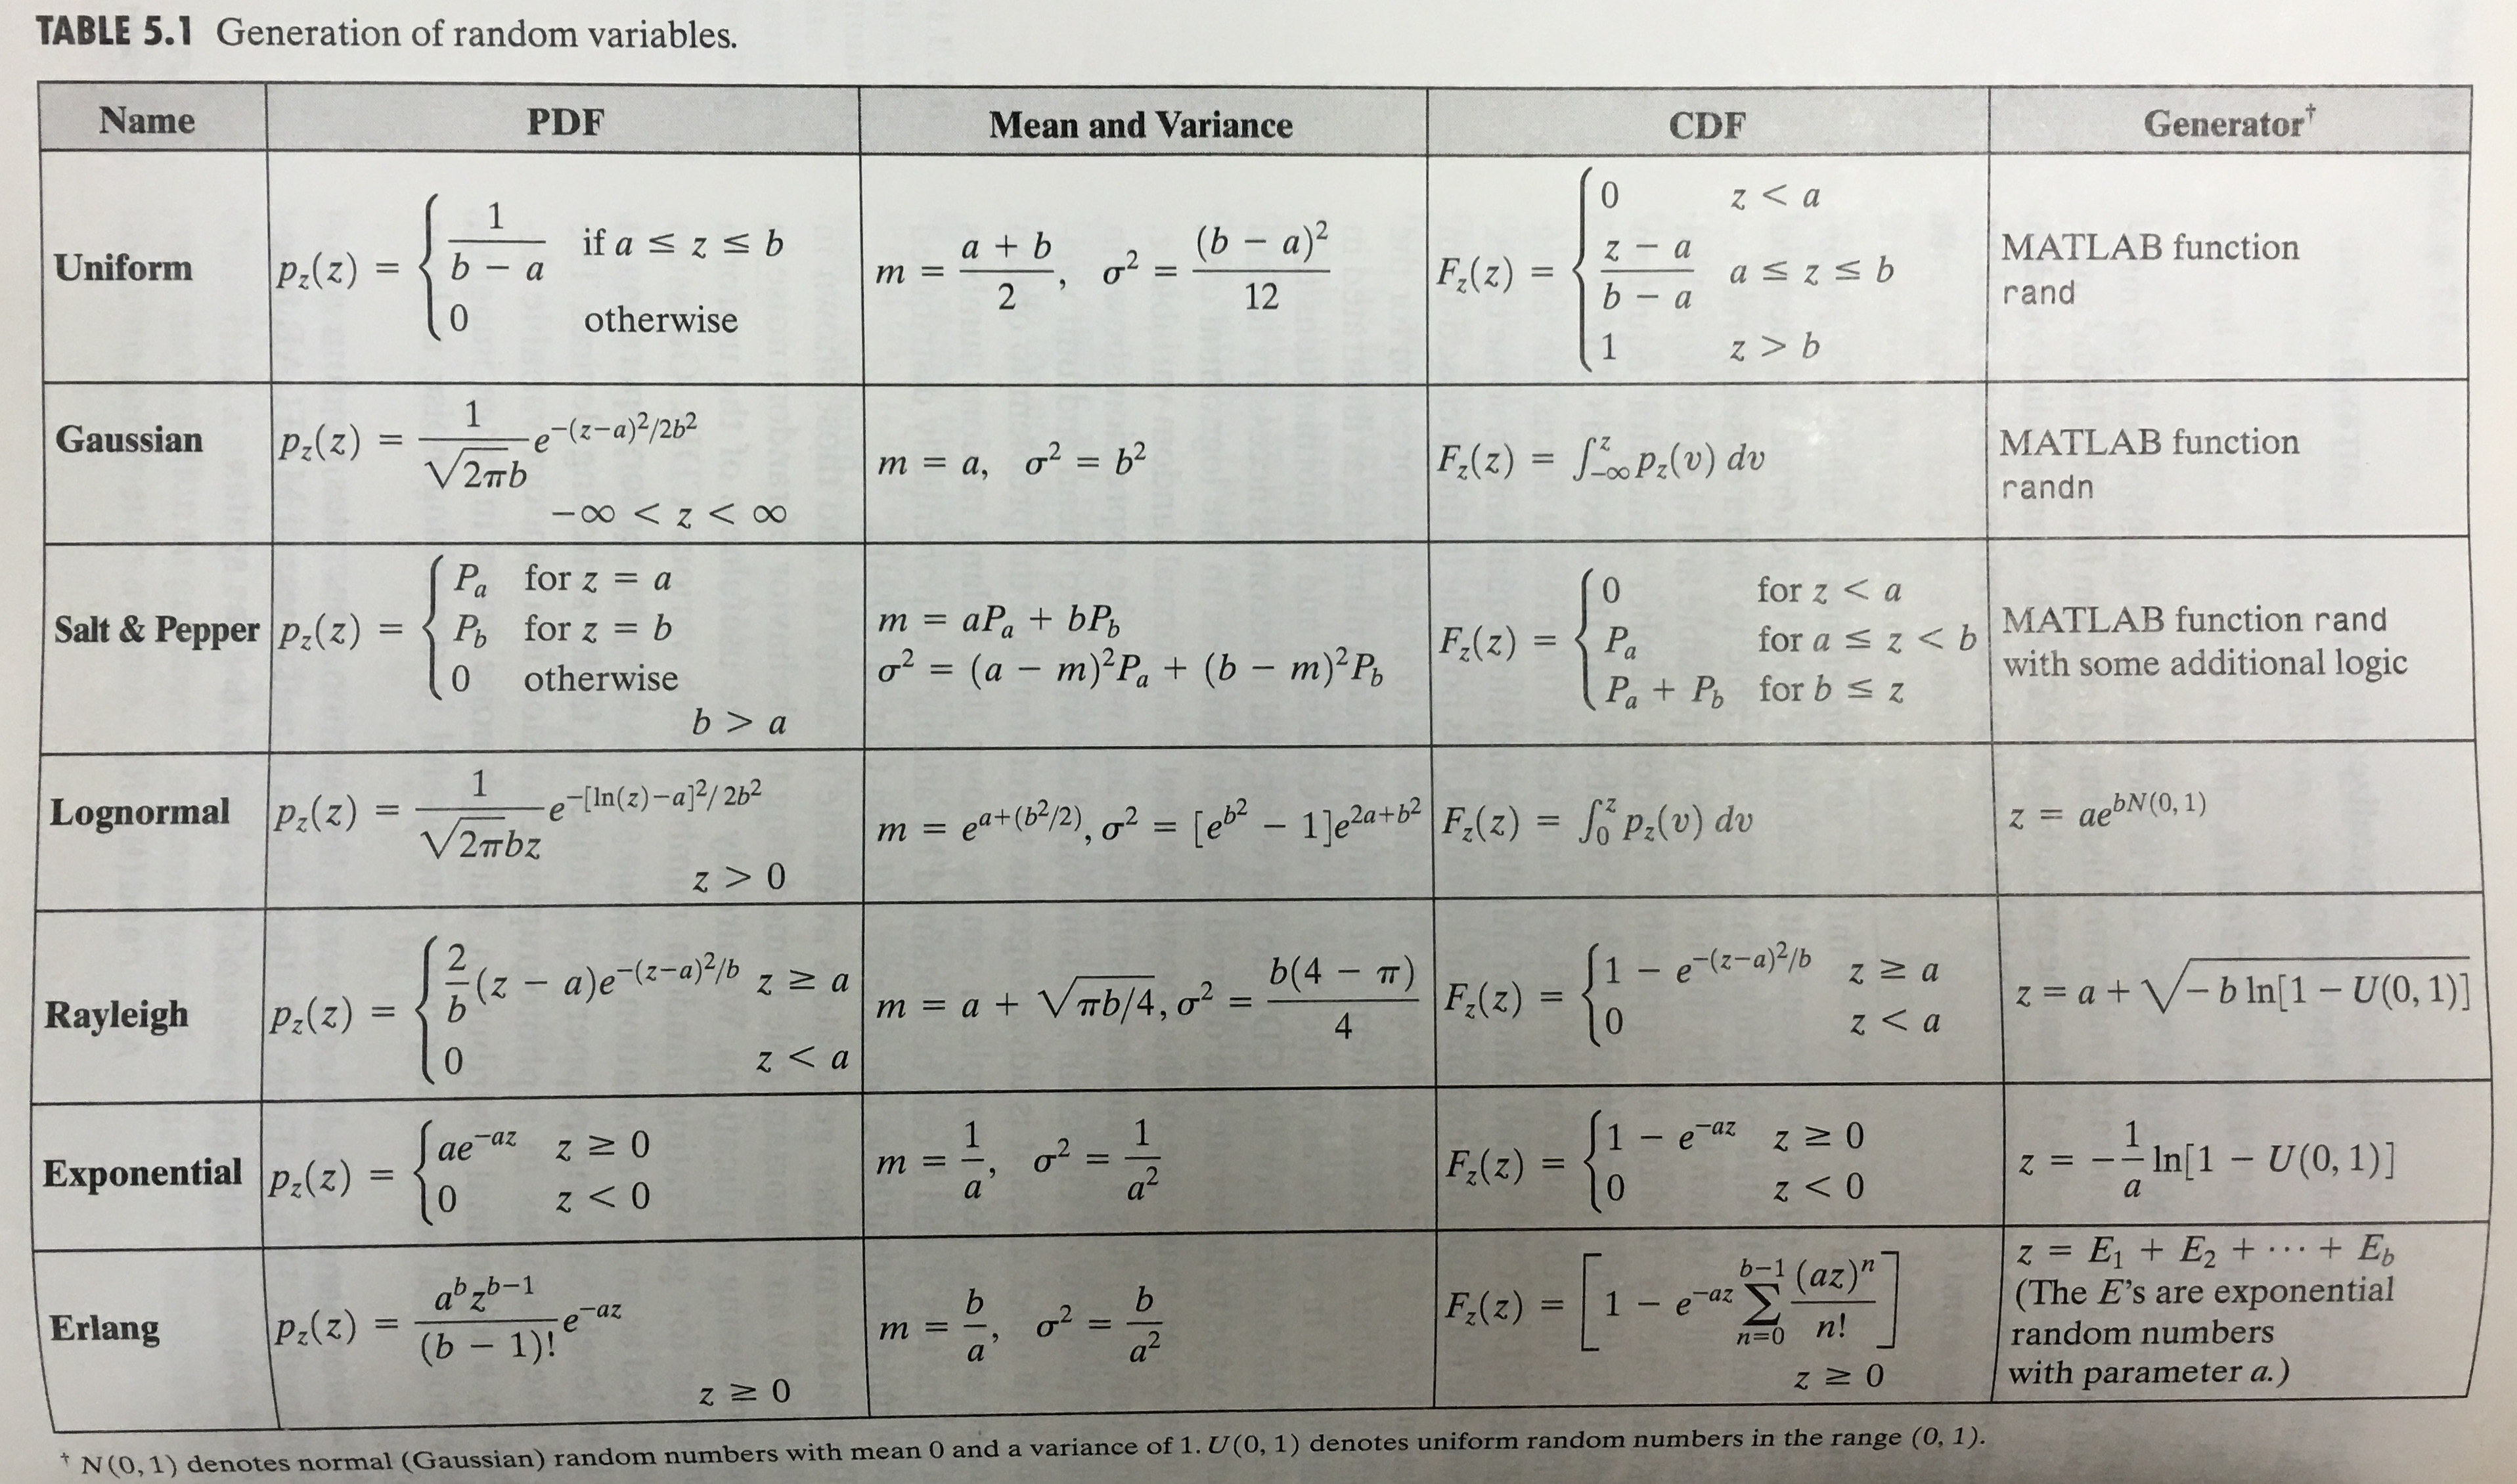
\includegraphics[scale=0.09]{pdf_cdf.jpg}
	\end{figure}
}
\frame
{
	\frametitle{Noise Integration}
	\selectlanguage{english}
	
	\begin{block}{Integration model}
		\begin{enumerate}
			\item Additive Noise
				\begin{itemize}
					\item Noise values will be \alert{\textbf{added}} to free-noise image to create image with noise.
					\item Model: $g(x,y) = f(x,y) + \eta(x,y)$
				\end{itemize}
				
			\item Multiplicative Noise
			\begin{itemize}
				\item Noise values will be \alert{\textbf{multiplied}} to free-noise image to create image with noise.
				\item Model: $g(x,y) = f(x,y) \times \eta(x,y)$
			\end{itemize}
			
		\end{enumerate}
	\end{block}
	\begin{alertblock}{}
		Each pixel in noise image $z = \eta(x,y)$ is generated according to previous algorithm to follow PDF $p_z(z)$
	\end{alertblock}
}
\begin{frame}[fragile]

	\frametitle{Noise generation}
	\selectlanguage{english}
	
	\begin{exercise}
		\begin{enumerate}
			\item Write a program to add noise (additive and multiplicative) to input image
		\end{enumerate}
	\end{exercise}
		
\end{frame}

\section{Noise Estimation}
\frame
{
	\frametitle{Noise Estimation}
	\selectlanguage{english}
	\begin{alertblock}{Reasons of estimation}
		\begin{itemize}
			\item Noise will be removed more effectively, if we know noise model in advance.
			\item So, noise reduction needs estimation of noise model
		\end{itemize}
	\end{alertblock}
}

\frame
{
	\frametitle{Noise Estimation: Methods}
	\selectlanguage{english}
	\begin{block}{Method of estimating noise model}
		\begin{enumerate}
			\item Select a small strip (called $S$) in input images. This trip contains reasonably constant gray level.
				\begin{itemize}
					\item "Reasonably" means gray levels are not too dark or bright
				\end{itemize}
			\item Compute histogram of values inside of the strip
			\item Observe the histogram to determine noise model
			\item Estimate the mean and the variance of PDF of noise model.
			\item Use the estimated mean and variance to estimate other parameters, for examples, $a$ and $b$ in other types of models different to Gaussian.
		\end{enumerate}
	\end{block}

}
\frame
{
	\frametitle{Noise Estimation: Methods}
	\selectlanguage{english}
	\begin{block}{Input data}
		\begin{enumerate}
			\item $S$ : a small strip in input image
			\item $p(z_i)$ : normalized histogram computed from $S$
		\end{enumerate}
	\end{block}
	\begin{alertblock}{Mean and Variance Estimation}
		\begin{enumerate}
			\item \alert{\textbf{Mean:}}
			\begin{align}
			\nonumber
			\mu = \sum_{z_i \in S}{z_{i}p(z_{i})}
			\end{align}
			
			\item \alert{\textbf{Variance:}}
			\begin{align}
			\nonumber
			\sigma^2 = \sum_{z_i \in S}{(z_{i-\mu)^2}p(z_{i})}
			\end{align}
		\end{enumerate}
	\end{alertblock}
}
\frame
{
	\frametitle{Noise Estimation: Example}
	\selectlanguage{english}
	\begin{example}
		\begin{figure}[!h]
			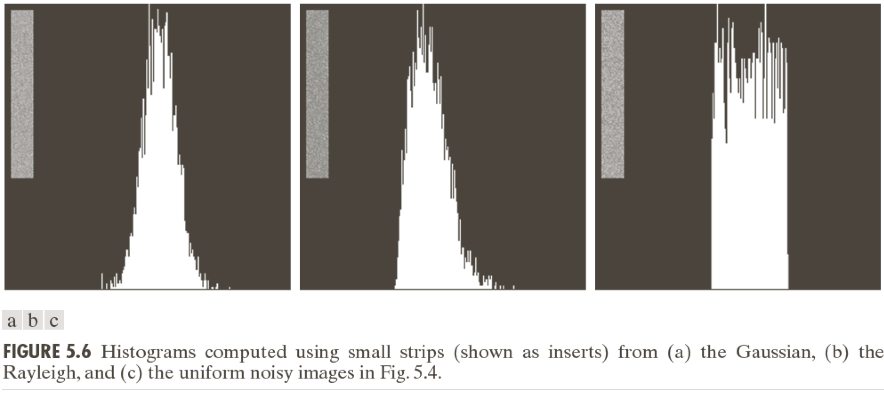
\includegraphics[scale=0.6]{noise_strip.png}
		\end{figure}
	\end{example}
	
}

\section{Mean filters}
\frame
{
	\Huge
	\begin{center}
		\textcolor{blue}{\textbf{Mean Filters}}
	\end{center}
}

\frame
{
	\frametitle{Mean filters: Arithmetic mean filter}
	\selectlanguage{english}
	
	\begin{block}{Mathematical model}
		\begin{align}
			\nonumber
			\hat{f}(x,y) = \frac{1}{mn}{\sum_{(s,t) \in S_{xy}} {g(s,t)}}
		\end{align}
	\end{block}
	\begin{alertblock}{Properties}
		\begin{enumerate}
			\item Smooth local variations in an image.
			\item Can reduce the following noises
				\begin{itemize}
					\item Additive Gaussian noise with zero mean
					\item Additive Uniform noise with zero mean
				\end{itemize}
			\item Result blurred image, especially, at edges,  with large $S_{xy}$.
		\end{enumerate}
	\end{alertblock}
	
}
\frame
{
	\frametitle{Mean filters: Geometric mean filter}
	\selectlanguage{english}
	
	\begin{block}{Mathematical model}
		\begin{align}
		\nonumber
		\hat{f}(x,y) = \left[ \prod_{(s,t) \in S_{xy}}{g(s,t)} \right]^{\frac{1}{mn}}
		\end{align}
	\end{block}
	\begin{alertblock}{Properties}
		\begin{enumerate}
			\item Smooth local variations in an image. Do smoothing comparable to the arithmetic mean filter
			\item Tend to lose less image detail
			\item Can reduce the following noises
			\begin{itemize}
				\item Additive Gaussian noise with zero mean
				\item Additive Uniform noise with zero mean
			\end{itemize}
			\item Result blurred image, especially, at edges, with large $S_{xy}$.
		\end{enumerate}
	\end{alertblock}
	
}
\frame
{
	\frametitle{Mean filters: Examples }
	\selectlanguage{english}
	\begin{figure}[!h]
		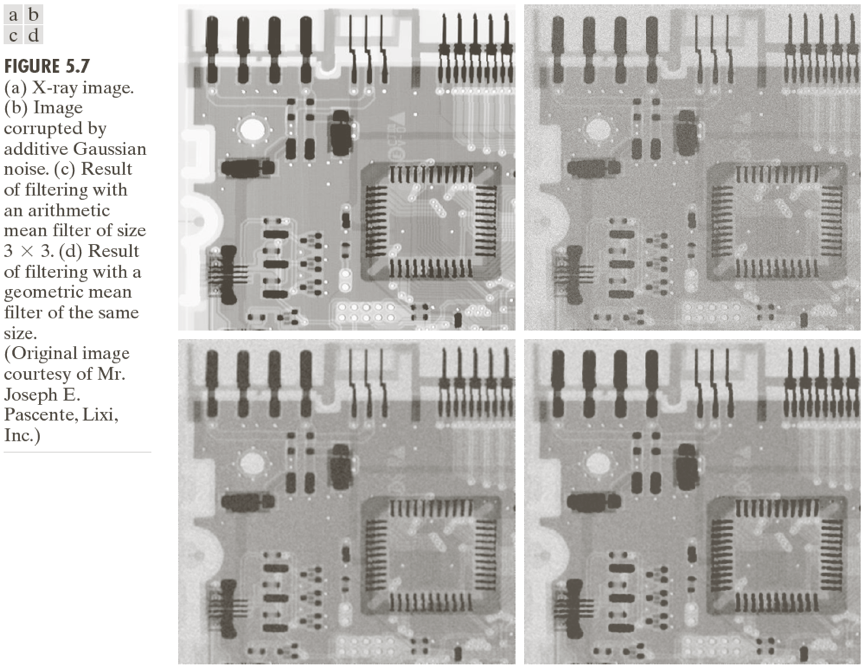
\includegraphics[scale=0.7]{arith_geo_mean.png}
	\end{figure}
	
}

\frame
{
	\frametitle{Mean filters: Harmonic mean filter}
	\selectlanguage{english}
	
	\begin{block}{Mathematical model}
		\begin{equation*}
		\nonumber
		\hat{f}(x,y) = \dfrac{mn}{\sum\limits_{(s,t) \in S_{xy}}{\dfrac{1}{g(s,t)}}}
		\end{equation*}
	\end{block}
	
	\begin{alertblock}{Properties}
		\begin{enumerate}
			\item Can reduce the following noises
			\begin{itemize}
				\item Additive Gaussian noise with zero mean
				\item Additive Uniform noise with zero mean
				\item Salt noise
			\end{itemize}
			\item Can not reduce pepper noise (black)
		\end{enumerate}
	\end{alertblock}
	
}
\frame
{
	\frametitle{Mean filters: Contraharmonic mean filter}
	\selectlanguage{english}
	
	\begin{block}{Mathematical model}
		\begin{equation*}
		\nonumber
		\hat{f}(x,y) = \dfrac{\sum\limits_{(s,t) \in S_{xy}}{g(s,t)^{Q+1}}}
		{\sum\limits_{(s,t) \in S_{xy}}{g(s,t)^Q}}
		\end{equation*}
		\begin{itemize}
			\item $Q$: order of the filter
			\item $Q=0$: Contraharmonic $\rightarrow$ Arithmetic
			\item $Q=1$: Contraharmonic $\rightarrow$ Harmonic
		\end{itemize}
	\end{block}
	
	\begin{alertblock}{Properties}
		\begin{enumerate}
			\item Can reduce pepper-and-salt noise
			\begin{itemize}
				\item $Q > 0$ : reduce pepper noise
				\item $Q < 0$ : reduce salt noise
			\end{itemize}
			\item Can not reduce pepper and salt noise simultaneously
		\end{enumerate}
	\end{alertblock}
	
}
\frame
{
	\frametitle{Mean filters: Examples }
	\selectlanguage{english}
	\begin{figure}[!h]
		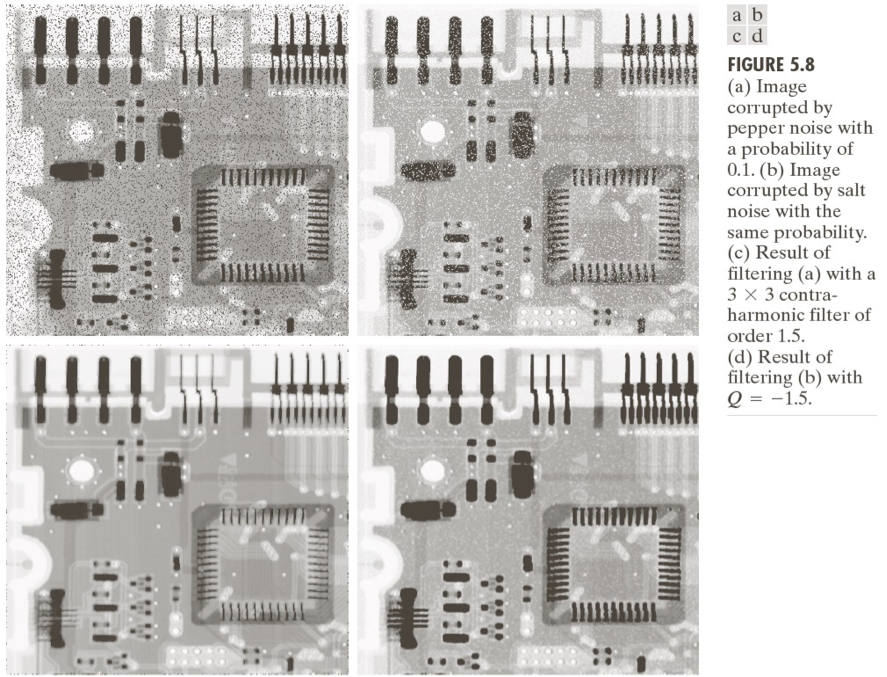
\includegraphics[scale=0.65]{contraharmonic_1.png}
	\end{figure}
	
}
\frame
{
	\frametitle{Mean filters: Examples }
	\selectlanguage{english}
	\begin{figure}[!h]
		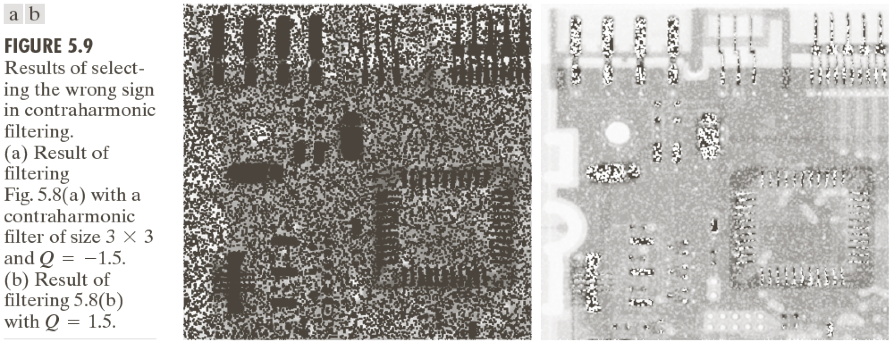
\includegraphics[scale=0.65]{contraharmonic_2.png}
	\end{figure}
	
}

\section{Order-Statistics Filters}
\frame
{
	\Huge
	\begin{center}
		\textcolor{blue}{\textbf{Order-Statistics Filters}}
	\end{center}
}

\frame
{
	\frametitle{Order-Statistics Filters: Median filter}
	\selectlanguage{english}
	
	\begin{block}{Mathematical model}
		\begin{align}
		\nonumber
		\hat{f}(x,y) = \underaccent{(s,t) \in S_{xy}}{\text{\alert{\textbf{median}}}}\{{g(s,t)}\}
		\end{align}
		
		\begin{itemize}
			\item Assign to the output image $\hat{f}(x,y)$ the median value of gray levels in the neighborhood of $(x,y)$
		\end{itemize}
		
	\end{block}
	\begin{alertblock}{Properties}
		\begin{enumerate}
			\item \alert{Effectively} reduce both of bipolar and unipolar impulse noise, i.e., \alert{salt-and-pepper noise}
			\item Produce less blurring images compared to linear 
			\item \alert{Can not} work with Gaussian noise
		\end{enumerate}
	\end{alertblock}
	
}
\frame
{
	\frametitle{Order-Statistics Filters: Examples }
	\selectlanguage{english}
	\begin{figure}[!h]
		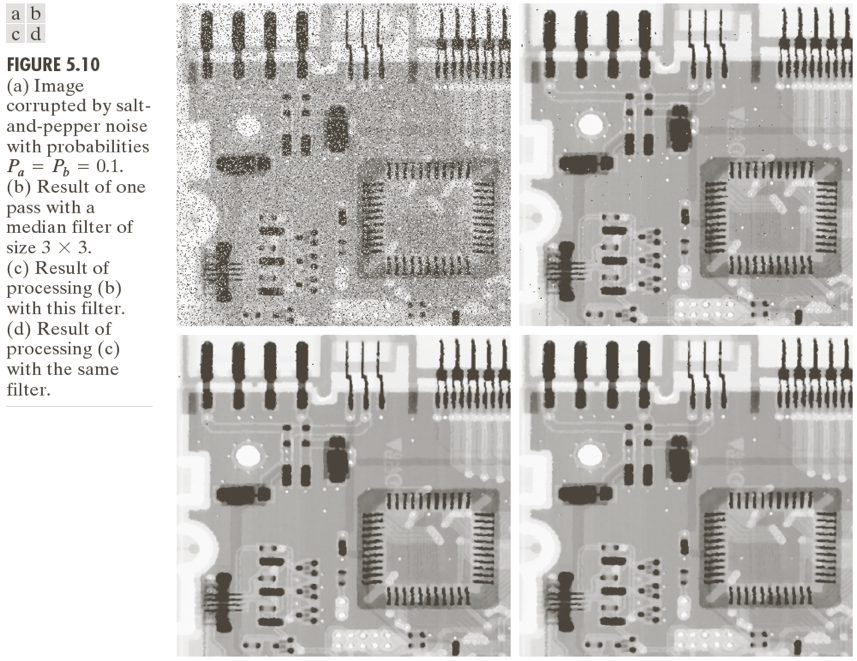
\includegraphics[scale=0.7]{median_demo.png}
	\end{figure}
	
}

\frame
{
	\frametitle{Order-Statistics Filters: Max and Min filter}
	\selectlanguage{english}
	
	\begin{block}{Mathematical model}
		\begin{align}
		\nonumber
		\hat{f}(x,y) = \underaccent{(s,t) \in S_{xy}}{\text{\alert{\textbf{max}}}}\{{g(s,t)}\} \\
		\nonumber
		\hat{f}(x,y) = \underaccent{(s,t) \in S_{xy}}{\text{\alert{\textbf{min}}}}\{{g(s,t)}\}
		\end{align}
		
		\begin{itemize}
			\item \alert{\textbf{Max filter}}: Assign to the output image $\hat{f}(x,y)$ the maximum value of gray levels in the neighborhood of $(x,y)$
			\item \alert{\textbf{Min filter}}: Assign to the output image $\hat{f}(x,y)$ the maximum value of gray levels in the neighborhood of $(x,y)$
		\end{itemize}
	\end{block}
}


\frame
{
	\frametitle{Order-Statistics Filters: Max and Min filter}
	\selectlanguage{english}
	\begin{block}{Mathematical model}
		\begin{align}
		\nonumber
		\hat{f}(x,y) = \underaccent{(s,t) \in S_{xy}}{\text{\alert{\textbf{max}}}}\{{g(s,t)}\} \\
		\nonumber
		\hat{f}(x,y) = \underaccent{(s,t) \in S_{xy}}{\text{\alert{\textbf{min}}}}\{{g(s,t)}\}
		\end{align}
	\end{block}
	\begin{alertblock}{Properties}
		\begin{enumerate}
			\item \alert{\textbf{Max filter}}: 
			\begin{itemize}
				\item Finds the brightest points in image
				\item Remove pepper noise
			\end{itemize}
			\item \alert{\textbf{Min filter}}:
			\begin{itemize}
				\item Finds the darkest points in image
				\item Remove salt noise
			\end{itemize}
		\end{enumerate}
	\end{alertblock}
}
\frame
{
	\frametitle{Order-Statistics Filters: Examples }
	\selectlanguage{english}
	\begin{figure}[!h]
		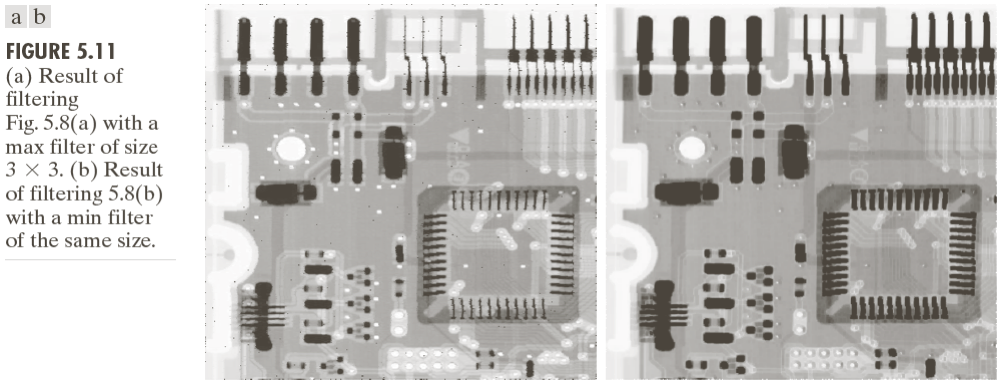
\includegraphics[scale=0.6]{max_min_demo.png}
	\end{figure}
	
}
\frame
{
	\frametitle{Order-Statistics Filters: Midpoint filter}
	\selectlanguage{english}
	\begin{block}{Mathematical model}
		\begin{align}
		\nonumber
		\hat{f}(x,y) = \frac{1}{2} \times { \left(\quad \underaccent{(s,t) \in S_{xy}}{\text{\alert{\textbf{max}}}}\{{g(s,t)}\}  \quad +  \quad \underaccent{(s,t) \in S_{xy}}{\text{\alert{\textbf{min}}}}\{{g(s,t)}\} \quad \right)}
		\end{align}
	\end{block}
	\begin{alertblock}{Properties}
		\begin{enumerate}
			\item Can reduce randomly distributed noise
			\begin{itemize}
				\item Additive Gaussian noise with zero mean
				\item Additive uniform noise with zero mean
			\end{itemize}
			
		\end{enumerate}
	\end{alertblock}
}
\frame
{
	\frametitle{Order-Statistics Filters: Alpha-trimmed mean filter}
	\selectlanguage{english}
	\begin{block}{Mathematical model}
		\begin{align}
		\nonumber
		\hat{f}(x,y) = \dfrac{1}{mn -d}{\sum\limits_{(s,t) \in S_{xy}}{g_{r}(s,t)}}
		\end{align}
		
		\begin{itemize}
			\item Delete $d/2$ lowest and $d/2$ highest gray values in neighborhood of $(x,y)$ to obtain $g_{r}(s,t)$ of $mn-d$ gray values.
			\item Assign the average of $g_{r}(s,t)$ to $\hat{f}(x,y)$
			\item $d = 0$: Alpha-trimmed $\rightarrow$ Arithmetic mean filter
			\item $d = (mn-1)/2$: Alpha-trimmed $\rightarrow$ Median filter
		\end{itemize}
	\end{block}
	\begin{alertblock}{Properties}
		\begin{enumerate}
			\item Useful in situations involving multiple types of noise, in combination of salt-and-pepper and Gaussian noise.
			
		\end{enumerate}
	\end{alertblock}
}
\frame
{
	\frametitle{Order-Statistics Filters: Examples }
	\selectlanguage{english}
	\begin{figure}[!h]
		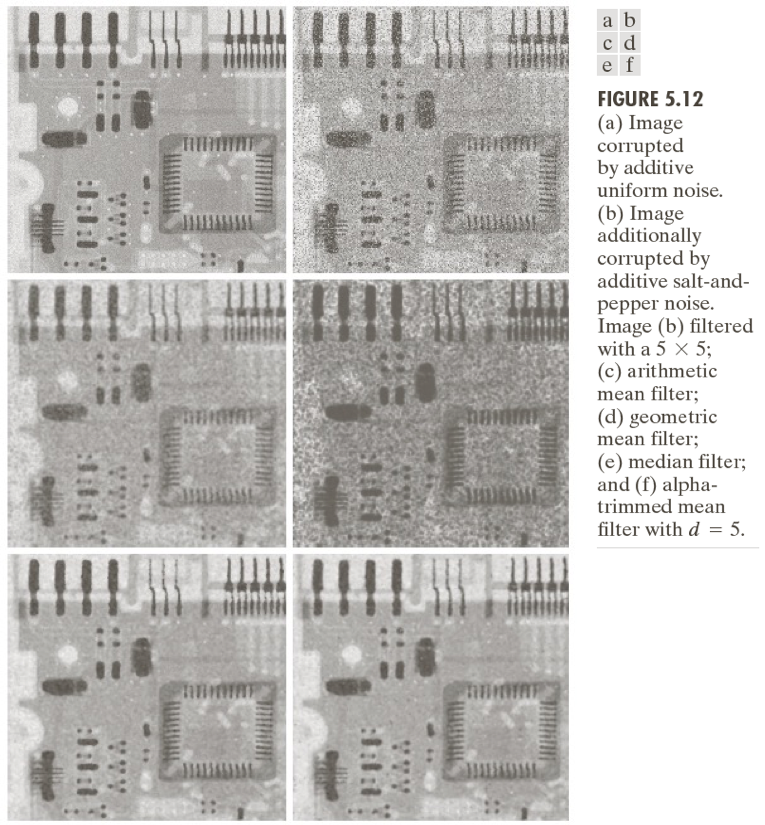
\includegraphics[scale=0.6]{alpha_trimmed.png}
	\end{figure}
	
}
\section{Image Restoration}
\frame
{
	\frametitle{Image Restoration: Model }
	\selectlanguage{english}
	\begin{figure}[!h]
		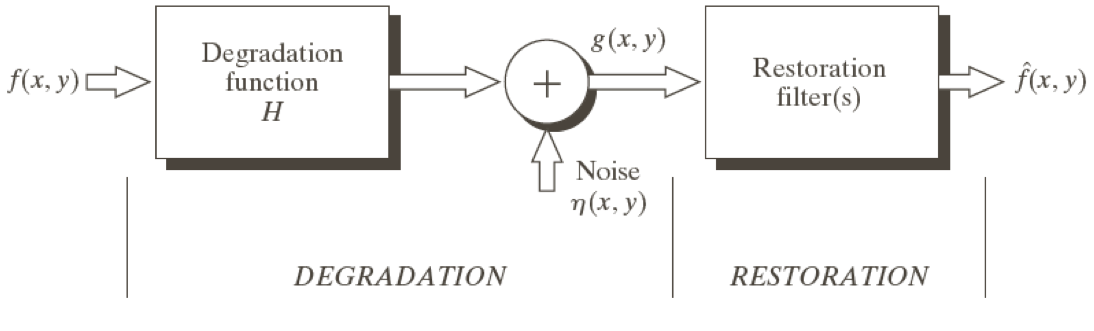
\includegraphics[scale=0.5]{degrad_restore.png}
		\caption{Model of degradation and restoration process}
	\end{figure}
	
	\begin{itemize}
		\item $f(x,y)$ : input image
		\item $\eta(x,y)$ : noise at $(x,y)$
		\item $\hat{f}(x,y)$ : restored image
	\end{itemize}
	
}
\frame
{
	\frametitle{Image Restoration: Model }
	\selectlanguage{english}
	\begin{block}{Linear, Position-Invariant Degradation}
		\begin{enumerate}
			\item Model in space domain:
		\end{enumerate}
		\begin{align}
			\nonumber
			g(x,y) &= h(x,y) * f(x,y) + \eta(x,y)
		\end{align}
		\begin{enumerate}
			\item Model in frequency domain:
		\end{enumerate}
		\begin{align}
		\nonumber
		G(u,v) &= H(u,v)F(u,v) + N(u,v)
		\end{align}
	\end{block}
	
	\begin{alertblock}{}
		$G(u,v)$, $H(u,v)$, $F(u,v)$, and $N(u,v)$ are \textbf{Fourier transforms} of $g(x,y)$, $h(x,y)$, $f(x,y)$ and  $\eta(x,y)$ respectively. 
	\end{alertblock}
}

\section{Inverse Filtering}
\frame
{
	\frametitle{Inverse Filtering }
	\selectlanguage{english}
	\begin{itemize}
		\item Let $\hat{F}(u,v$ be estimate of Fourier transforms of $f(x,y)$
	\end{itemize}
	
	\begin{block}{Ideal Restoration}
		\begin{align}
		\nonumber
		\hat{F}(u,v)  &= \dfrac{G(u,v)}{H(u,v)} \\
		\nonumber
				&= F(u,v) + \dfrac{N(u,v)}{H(u,v)}
		\end{align}
	\end{block}
	\begin{alertblock}{Problems}
		\begin{enumerate}
			\item \alert{\textbf{Problem 1}}: even you know $H(u,v)$, you can not recover $f(x,y)$ exactly because you do not know $N(u,v)$.
			\item \alert{\textbf{Problem 2}}: At some $(u,v)$, $H(u,v) = 0$ will cause $N(u,v)/H(u,v)$ to dominate $\hat{F}(u,v)$.
		\end{enumerate}
	\end{alertblock}
}
\frame
{
	\frametitle{Inverse Filtering }
	\selectlanguage{english}
	
	\begin{block}{Inverse Filtering}
		\begin{align}
		\nonumber
		\hat{F}(u,v)  &= \dfrac{G(u,v)}{H(u,v)}
		\end{align}
	\end{block}
	\begin{alertblock}{Tools for existing problems}
		\begin{enumerate}
			\item \alert{\textbf{Problem 1}}: Assume that there is no noise.
			\item \alert{\textbf{Problem 2}}: At some $(u,v)$, $H(u,v) = 0$:
				\begin{enumerate}
					\item \alert{\textbf{Replacement:}} Replace $H(u,v) =$ a certain value at $(u,v)$ where $H(u,v) = 0$:
					\item \alert{\textbf{Cut-off:}} Filter $G(u,v)/H(u,v)$ with Butterworth lowpass function of some order, e.g., order $=10$, with some radius, e.g., $40, 70$, etc - dependent on image size.
					\item \alert{\textbf{Finding radius:}} Go from the origin to outside radially, find the first $(u,v)$ that $H(u,v) = 0$. Limit the filter frequencies from the origin to this radius.
				\end{enumerate}
		\end{enumerate}
	\end{alertblock}
}
\frame
{
	\frametitle{Inverse Filtering: Demonstration }
	\selectlanguage{english}
	\begin{figure}[!h]
		\begin{tabular}{cc}
			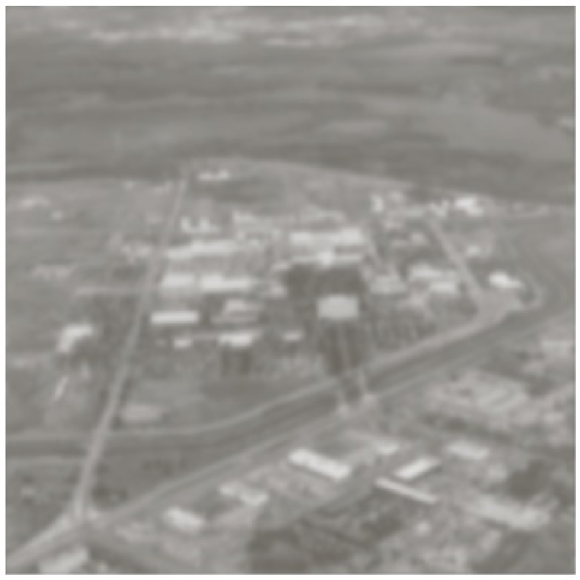
\includegraphics[height=4.5cm]{inverse_filter_original.png} &
			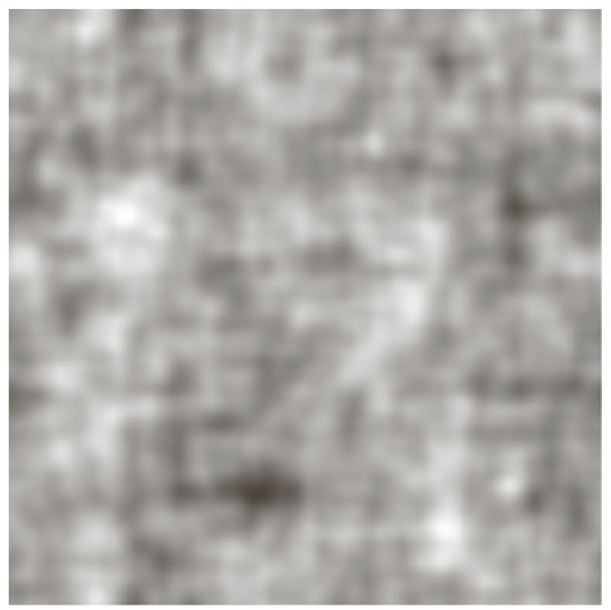
\includegraphics[height=4.5cm]{inverse_filter_full.png} \\
			(a) Original image & (b) Cut-off, $R$=full\\
		\end{tabular}
	\end{figure}
}
\frame
{
	\frametitle{Inverse Filtering: Demonstration }
	\selectlanguage{english}
	\begin{figure}[!h]
		\begin{tabular}{cc}
			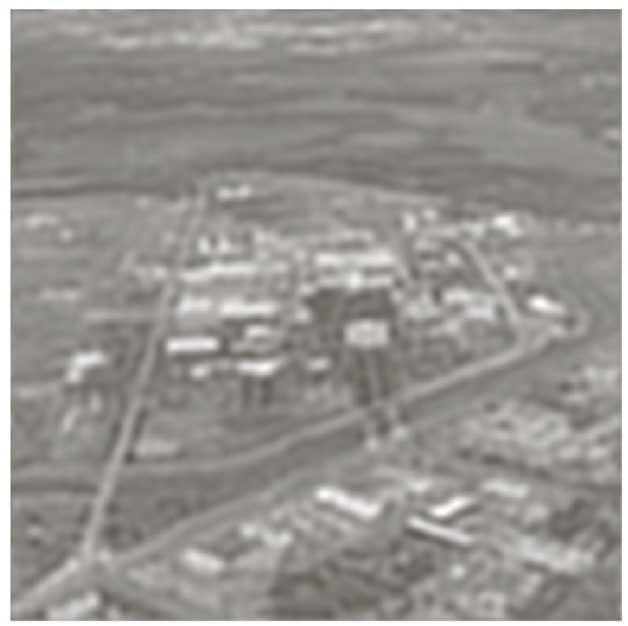
\includegraphics[height=4.5cm]{inverse_filter_off_r40.png} &
			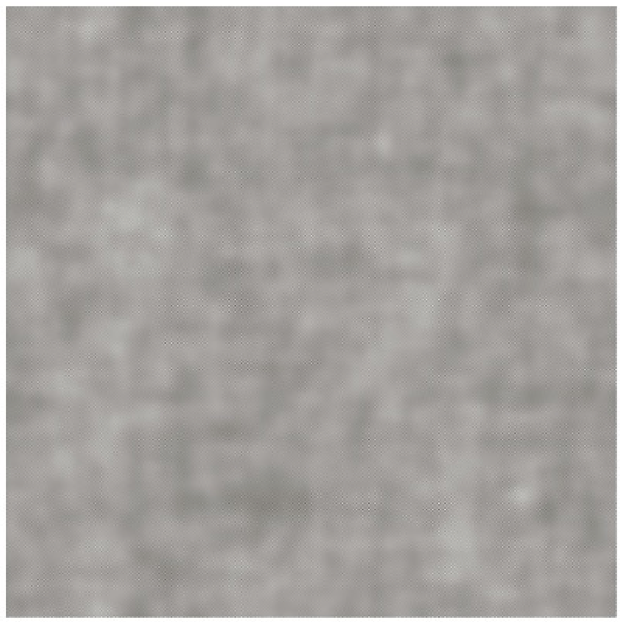
\includegraphics[height=4.5cm]{inverse_filter_off_r85.png} \\
			(a) Cut-off, $R=40$ & (b) Cut-off, $R=85$\\
		\end{tabular}
	\end{figure}
}
\frame
{
	\frametitle{Inverse Filtering: Demonstration }
	\selectlanguage{english}
	\begin{figure}[!h]
		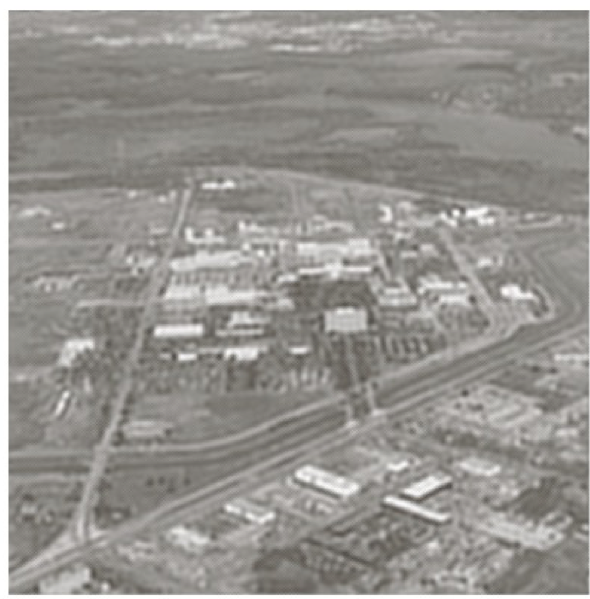
\includegraphics[height=7.5cm]{inverse_filter_off_r70.png}
		\caption{Cut-off, $R=70$}
	\end{figure}
}
\begin{frame}[fragile]
	\frametitle{Inverse Filtering: Demonstration }
	\selectlanguage{english}
	
	\begin{exercise}
		\begin{enumerate}
			\item Write a program to simulate the atmospheric turbulence phenomenon, modeled by $H(u,v)$ in frequency domain as in the following. Take a look at Gonzalez's Book, page 258.
			\begin{align}
			\nonumber
				H(u,v) &= e^{-k(u^2 + v^2)^5/6}
			\end{align}
			\begin{itemize}
				\item Some $k$: $k = 0.001, 0.0025, 0.00025$
			\end{itemize}
			
			\item Write a program to remove the atmospheric turbulence phenomenon from images (generated from previous question.)
		\end{enumerate}
	\end{exercise}
		
\end{frame}

\section{Wiener Filtering}
\frame
{
	\frametitle{Wiener Filtering }
	\selectlanguage{english}
	
	\begin{block}{Names and Wiener Filter's objective}
		\begin{itemize}
			\item Other name: Minimum Mean Square Error Filter
			\item Objective: to minimize the mean square error between uncorrupted image $f$ and its estimate $\hat{f}$.
			\item $\equiv$ Minimize 
		\end{itemize}
			\begin{align}
				\nonumber
				e^2 = E\{(f - \hat{f})^2\}
			\end{align}
	\end{block}

}
\frame
{
	\frametitle{Wiener Filtering }
	\selectlanguage{english}
	\small{
	\begin{block}{Mathematical Model}
		\begin{align}
			\nonumber
			\hat{F}(u,v) = \left[ \dfrac{1}{H(u,v)} \times 
				\dfrac{|H(u,v)|^2}{|H(u,v)|^2 + S_{\eta}(u,v)/S_{f}(u,v)}\right]G(u,v)
		\end{align}
	\end{block}
	
	\begin{block}{}
		\begin{itemize}
			\item $H(u,v)$ : degradation function (assume that it has been estimated).
			\item $G(u,v)$ : Fourier transforms of degraded image $g(x,y)$, can be computed.
			\item $|H(u,v)|^2 = H^{*}(u,v)H(u,v)$: power spectrum of degradation function, can be computed
			\item $S_{\eta}(u,v) = |N(u,v)|^2$: power spectrum of noise.
			\item $S_{f}(u,v) = |F(u,v)|^2$: power spectrum of uncorrupted image. \textbf{This seldom is  known}.
		\end{itemize}.
	\end{block}
}
}
\frame
{
	\frametitle{Wiener Filtering }
	\selectlanguage{english}
	\small{
	\begin{block}{Mathematical Model}
		\begin{align}
		\nonumber
		\hat{F}(u,v) = \left[ \dfrac{1}{H(u,v)} \times 
		\dfrac{|H(u,v)|^2}{|H(u,v)|^2 + S_{\eta}(u,v)/S_{f}(u,v)}\right]G(u,v)
		\end{align}
	\end{block}
	}
	
	\begin{block}{Wiener filter to Inverse filter}
		Sepcial case: There is no noise. $N(u,v) = 0$. 
		
		Wiener filtering becomes Inverse filtering.
		
	\end{block}
}
\frame
{
	\frametitle{Wiener Filtering }
	\selectlanguage{english}
	
	\begin{block}{A special case - White noise}
		We do not know:
		\begin{enumerate}
			\item $S_{\eta}(u,v)$ : power spectrum of noise
			\item $S_{f}(u,v)$ : power spectrum of input signal
		\end{enumerate}
		For white noise, we hope that, at a specific frequency $(u,v)$, the power of noise is proportional to the power of input signal. It means $S_{\eta}(u,v) = K \times S_{f}(u,v)$
	
		\begin{align}
			\nonumber
			\dfrac{ S_{\eta}(u,v)}{S_{f}(u,v)} = K 
		\end{align}

	\end{block}
	\begin{alertblock}{Remind}
		White noise is a type of noise that affects on all frequencies.
	\end{alertblock}
}
\frame
{
	\frametitle{Wiener Filtering }
	\selectlanguage{english}
	
	\begin{block}{Mathematical Model for white noise}
		\begin{align}
		\nonumber
		\hat{F}(u,v) = \left[ \dfrac{1}{H(u,v)} \times 
		\dfrac{|H(u,v)|^2}{|H(u,v)|^2 + K}\right]G(u,v)
		\end{align}
	\end{block}
	
}

\frame
{
	\frametitle{Wiener Filtering: Demonstration }
	\selectlanguage{english}
	
	\begin{alertblock}{Demonstration's model of degradation}
		The demonstration for Wiener filtering in some consecutive slides uses \alert{\textbf{motion blur}} degradation model, as shown below.
		
		\begin{align}
			\nonumber
			H(u,v) &= \dfrac{T}{\pi(ua + vb)} sin\left[\pi(ua + vb)\right]e^{-j\pi(ua + vb)}
		\end{align}
		
		\begin{itemize}
			\item $a = b = 0.1$
			\item $T = 1$
		\end{itemize}
	\end{alertblock}
}
\frame
{
	\frametitle{Wiener Filtering: Demonstration }
	\selectlanguage{english}
	
	\begin{figure}[!h]
		\begin{tabular}{cc}
			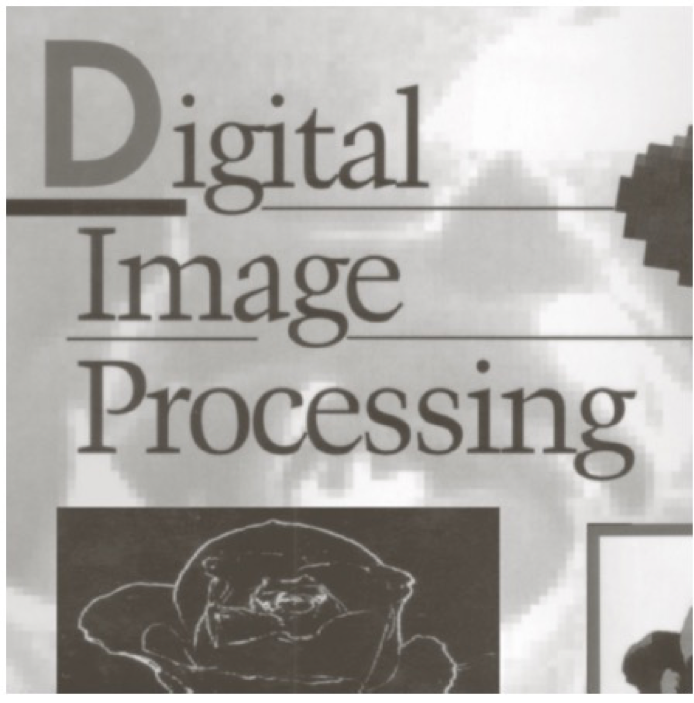
\includegraphics[height=4.5cm]{book_original.png} &
			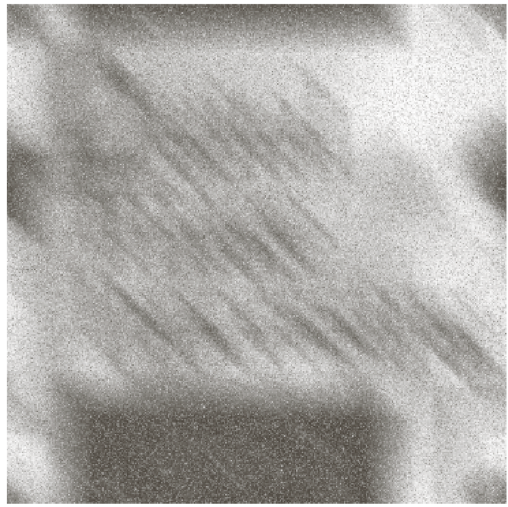
\includegraphics[height=4.5cm]{book_degrad_1.png} \\
			(a) Original image & (b) Degraded image\\
		\end{tabular}
	\end{figure}
	\begin{block}{Degradation method}
		\begin{enumerate}
			\item Blurring the original with motion model
			\item Corrupting heavily with additive Gaussian noise, zeros mean, variance of 650
		\end{enumerate}
	\end{block}
}
\frame
{
	\frametitle{Wiener Filtering: Demonstration }
	\selectlanguage{english}
	
	\begin{figure}[!h]
		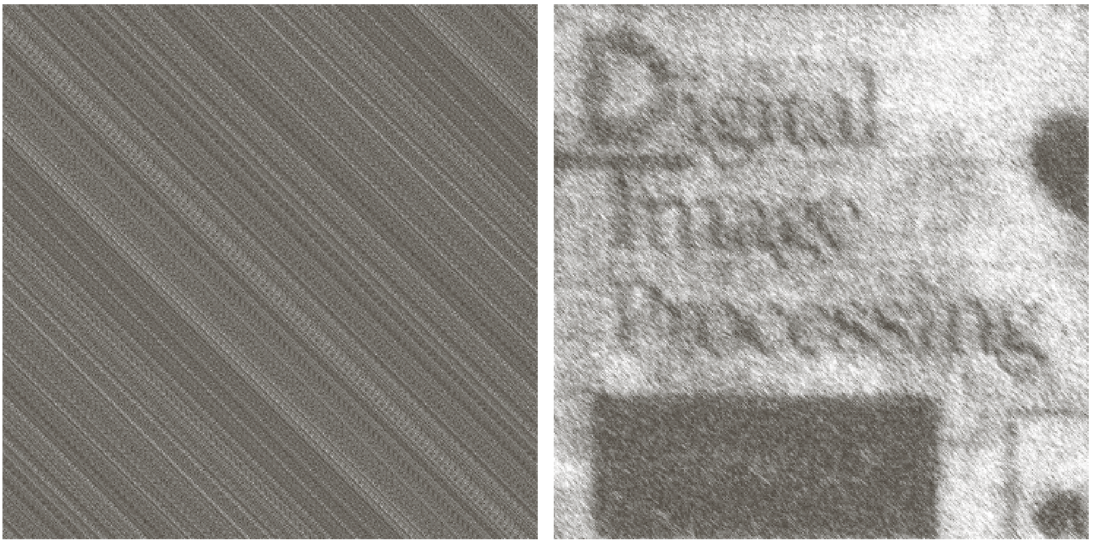
\includegraphics[width=10cm]{book_restore_1.png}
		\caption{Restored images. Left: \alert{Inverse Filtering}, Right: \alert{Wiener Filtering}, $K$ is selected to for best result}
	\end{figure}

}

\frame
{
	\frametitle{Wiener Filtering: Demonstration }
	\selectlanguage{english}
	
	\begin{figure}[!h]
		\begin{tabular}{cc}
			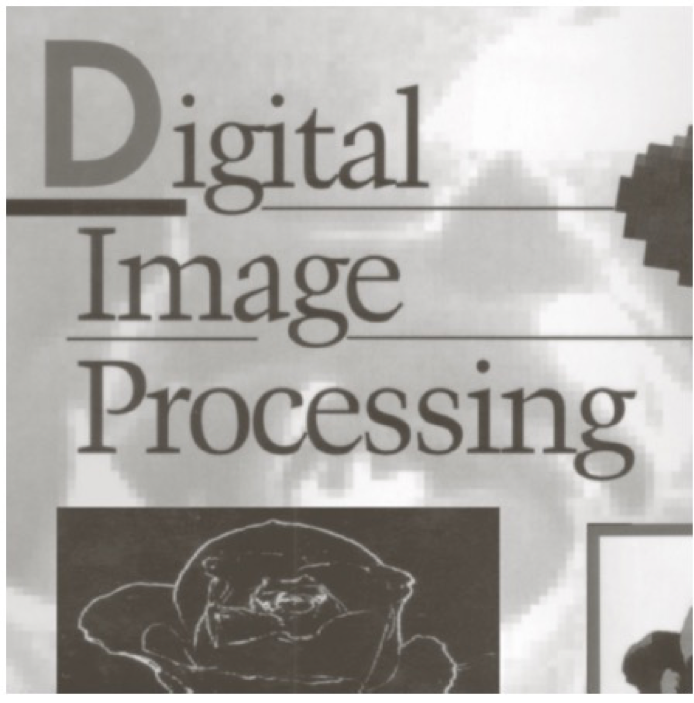
\includegraphics[height=4.5cm]{book_original.png} &
			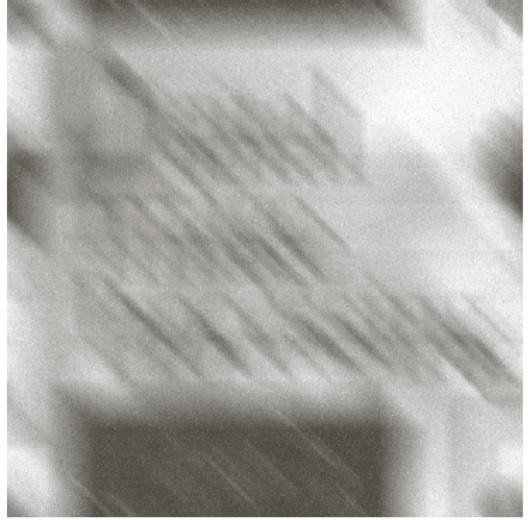
\includegraphics[height=4.5cm]{book_degrad_2.png} \\
			(a) Original image & (b) Degraded image\\
		\end{tabular}
	\end{figure}
	\begin{block}{Degradation method}
		\begin{enumerate}
			\item Blurring the original with motion model
			\item Corrupting additive Gaussian noise with smaller variance compared to the previous case, zeros mean.
		\end{enumerate}
	\end{block}
}
\frame
{
	\frametitle{Wiener Filtering: Demonstration }
	\selectlanguage{english}
	
	\begin{figure}[!h]
		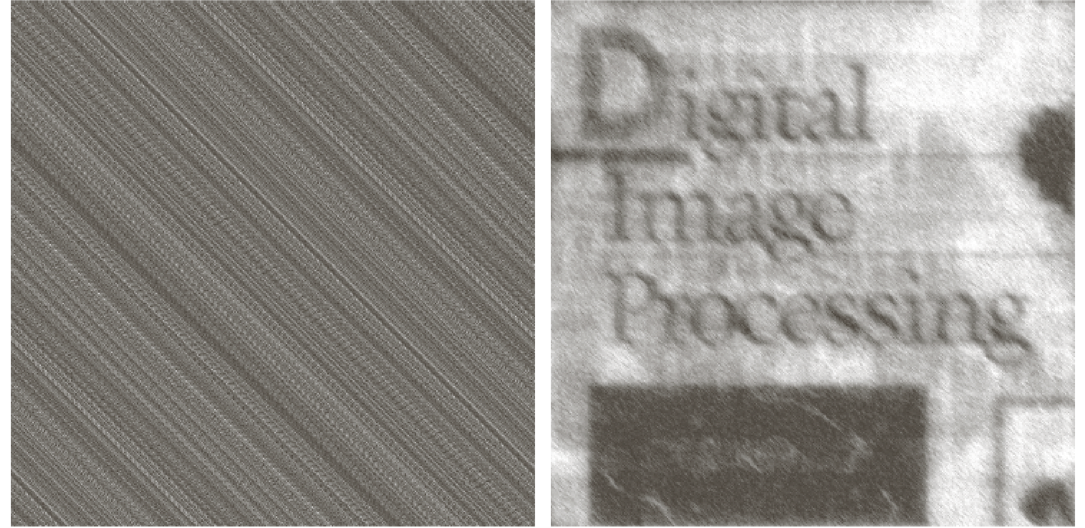
\includegraphics[width=10cm]{book_restore_2.png}
		\caption{Restored images. Left: \alert{Inverse Filtering}, Right: \alert{Wiener Filtering}, $K$ is selected to for best result}
	\end{figure}
	
}
\frame
{
	\frametitle{Wiener Filtering: Demonstration }
	\selectlanguage{english}
	
	\begin{figure}[!h]
		\begin{tabular}{cc}
			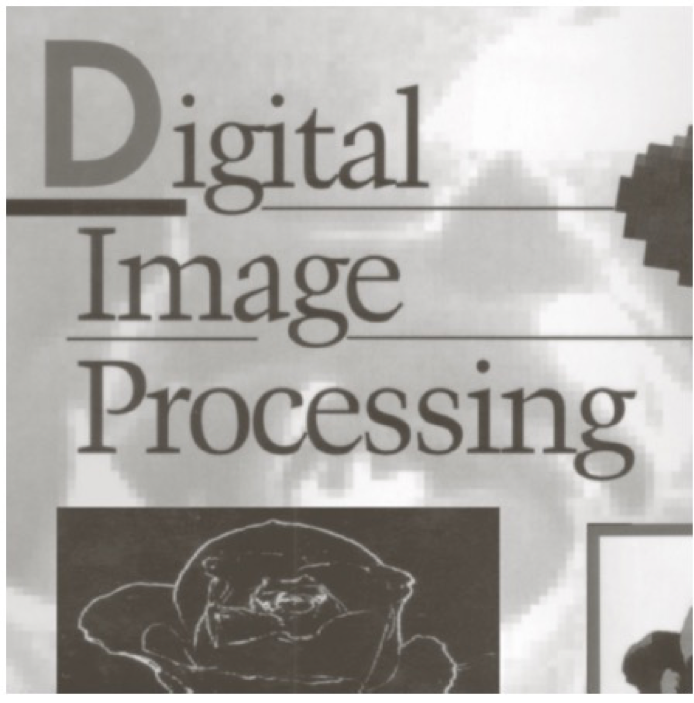
\includegraphics[height=4.5cm]{book_original.png} &
			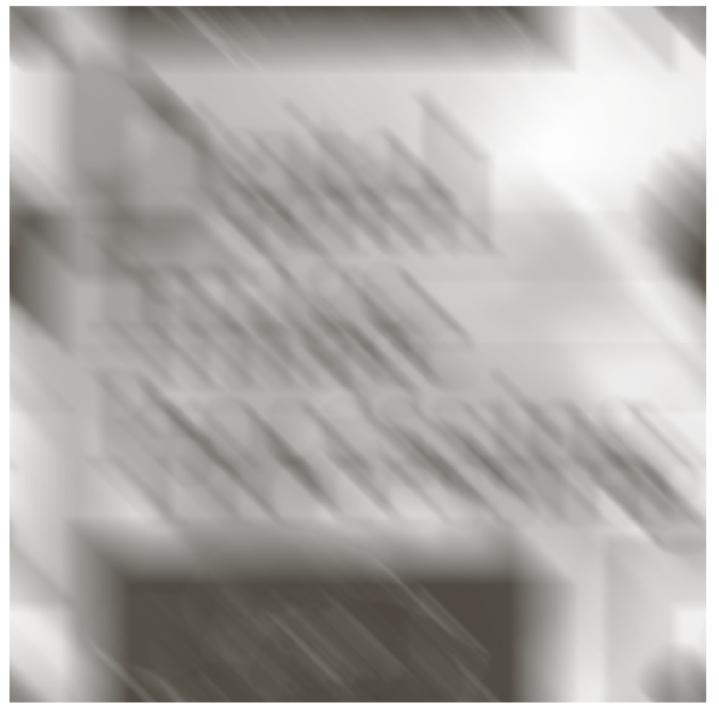
\includegraphics[height=4.5cm]{book_degrad_3.png} \\
			(a) Original image & (b) Degraded image\\
		\end{tabular}
	\end{figure}
	\begin{block}{Degradation method}
		\begin{enumerate}
			\item Blurring the original with motion model
			\item Corrupting additive Gaussian noise with smaller variance compared to the previous case, zeros mean.
		\end{enumerate}
	\end{block}
}
\frame
{
	\frametitle{Wiener Filtering: Demonstration }
	\selectlanguage{english}
	
	\begin{figure}[!h]
		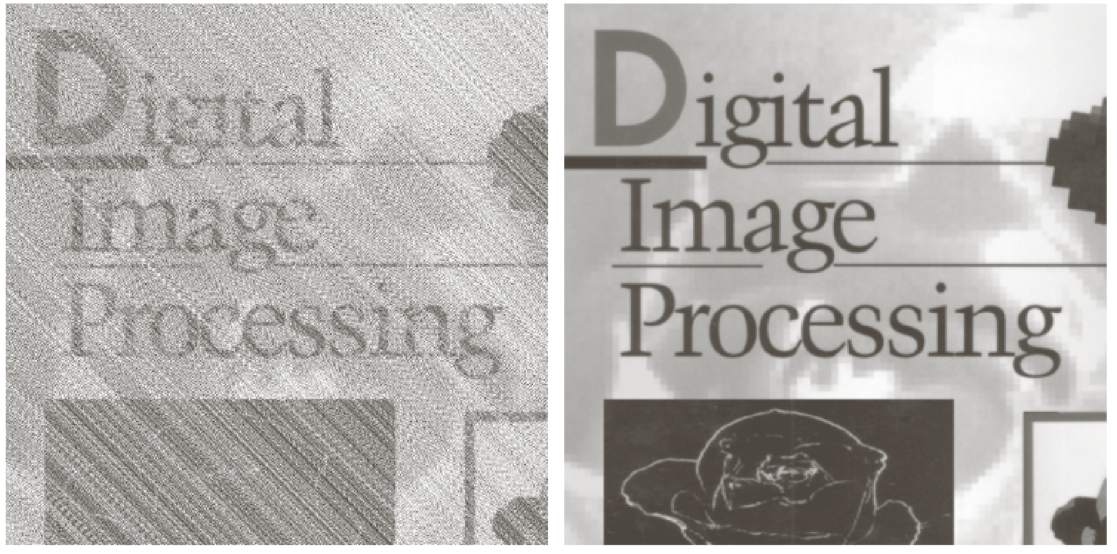
\includegraphics[width=10cm]{book_restore_3.png}
		\caption{Restored images. Left: \alert{Inverse Filtering}, Right: \alert{Wiener Filtering}, $K$ is selected to for best result}
	\end{figure}
	\begin{itemize}
		\item The result of Wiener filter in this case shows excellent quality!
	\end{itemize}
}
\begin{frame}[fragile]
	\frametitle{Wiener Filtering: Exercises }
	\selectlanguage{english}
	
	\begin{exercise}
		\begin{enumerate}
			\item Write a program to degrade input images with motion blur model and additive Gaussian noise with zeros mean.
			\item Write a program to restore degraded images with Wiener and Inverse filtering
		\end{enumerate}
	\end{exercise}
\end{frame}

%%%%%%%%%%%%%%%%%%%%%%%%%%%%%%%%%%%%%%%%%%%%%%%

%%%%%%%%%%%%%%%%%%%%%%%%%%%%%%%%%%%%%%%%%%%%%%%

\end{document}